\documentclass{beamer}

\usepackage[utf8]{inputenc}
\usepackage{amsmath,amsfonts,amssymb}
\usepackage{listings}
\usepackage{graphicx}
\usepackage{tikz}
\usetikzlibrary{arrows.meta,positioning}
\usepackage{hyperref}
\usepackage{booktabs}

\graphicspath{{../}{./}{../images/}{./images/}}

% ===== KCPC clean theme (Weeks 1, 2, 3, and Year 2) =====
\usetheme{default}
\useinnertheme{rectangles}
\useoutertheme{default}
\setbeamertemplate{navigation symbols}{}

\definecolor{kcpc-bg}{RGB}{250,250,250}
\definecolor{kcpc-text}{RGB}{20,20,20}
\definecolor{kcpc-muted}{RGB}{90,90,90}
\definecolor{kcpc-red}{RGB}{176,0,0}
\definecolor{kcpc-blue}{RGB}{0,90,170}
\definecolor{kcpc-amber}{RGB}{190,115,0}
\definecolor{kcpc-green}{RGB}{20,130,60}

\setbeamercolor{background canvas}{bg=kcpc-bg}
\setbeamercolor{normal text}{fg=kcpc-text}
\setbeamercolor{frametitle}{fg=kcpc-text,bg=kcpc-bg}
\setbeamercolor{title}{fg=kcpc-text}
\setbeamercolor{subtitle}{fg=kcpc-muted}
\setbeamercolor{structure}{fg=kcpc-red}
\setbeamerfont{title}{series=\bfseries,size=\Large}
\setbeamerfont{frametitle}{series=\bfseries,size=\large}
\setlength{\parskip}{0.35em}

\setbeamertemplate{itemize item}{$\rightarrow$}
\setbeamertemplate{itemize subitem}{$\rightarrow$}
\setbeamertemplate{headline}{\vspace{0.2cm}\hspace{0.2cm}\textcolor{kcpc-muted}{\small\insertsection}\hfill}
\setbeamertemplate{footline}{\hspace{0.2cm}\textcolor{kcpc-muted}{\small KCPC}\hfill\vspace{0.3cm}}
\setbeamertemplate{background}{%
  \begin{tikzpicture}[remember picture,overlay]
    \node[opacity=0.035,at=(current page.center)]
      {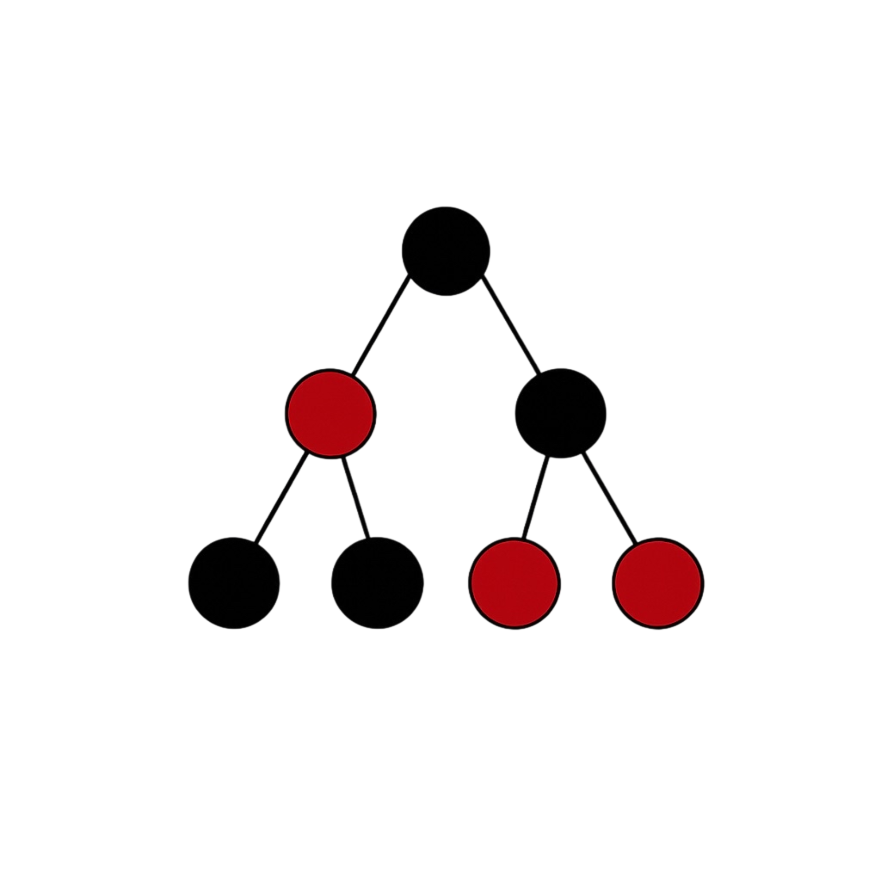
\includegraphics[width=0.55\paperwidth]{kcpc-logo.png}};
  \end{tikzpicture}%
}
\AtBeginSection[]{\begin{frame}[plain]\vfill\centering{\Large\bfseries\insertsection}\vfill\end{frame}}
\hypersetup{colorlinks=true,linkcolor=kcpc-red,urlcolor=kcpc-red}

\lstset{
  basicstyle=\ttfamily\scriptsize,
  keywordstyle=\bfseries\color{kcpc-red},
  commentstyle=\itshape\color{kcpc-muted},
  columns=fullflexible,
  keepspaces=true,
  showstringspaces=false,
  frame=single,
  rulecolor=\color{kcpc-muted}
}

\tikzset{
  gnode/.style={circle,draw=kcpc-text,thick,minimum size=16pt,inner sep=1pt,font=\scriptsize\bfseries,fill=white},
  active/.style={circle,draw=kcpc-blue,very thick,minimum size=16pt,inner sep=1pt,font=\scriptsize\bfseries,fill=kcpc-blue!15},
  done/.style={circle,draw=kcpc-red,very thick,minimum size=16pt,inner sep=1pt,font=\scriptsize\bfseries,fill=kcpc-red!12},
  treeedge/.style={draw=kcpc-blue,very thick},
  backedge/.style={draw=kcpc-amber,very thick,dashed}
}

\title{Introduction to Graphs}
\subtitle{Representations, Traversals, and Structural Patterns}
\author{King's Competitive Programming Club}
\date{Workshop 4}

\begin{document}

\begin{frame}[plain]\titlepage\end{frame}

\begin{frame}{Workshop Overview}
  \begin{enumerate}
    \item Graph Definitions and Structural Families
    \item Storing Graphs: Representations and Trade-Offs
    \item Breadth-First Search (BFS) and Unweighted Shortest Paths
    \item Depth-First Search (DFS) and Edge Classification
    \item Core Algorithmic Patterns for the Problem Sheet
    \item Conclusion and Try-It-Yourself Solutions
  \end{enumerate}
\end{frame}

% ============================================================
\section{Graph Definitions and Structural Families}
% ============================================================

\begin{frame}{What Is a Graph?}
  \begin{columns}[c]
    \begin{column}{0.56\textwidth}
      A \textbf{graph} $G = (V, E)$ consists of:
      \begin{itemize}
        \item A set of \textbf{vertices} (nodes) $V = \{1, 2, \dots, n\}$.
        \item A set of \textbf{edges} $E$ connecting pairs of vertices.
      \end{itemize}
      \textbf{Example:} $V = \{1,2,3,4,5,6\}$,\\[2pt]
      {\small $E = \{(1,2), (1,3), (2,3), (4,2), (6,5)\}$.}
      \begin{itemize}
        \item \textbf{Undirected:} edges are two-way $\{u,v\}$.
        \item \textbf{Directed:} edges are one-way arrows $(u \to v)$.
      \end{itemize}
    \end{column}
    \begin{column}{0.42\textwidth}
      \centering
      {\scriptsize\textbf{Undirected graph}}\\[2pt]
      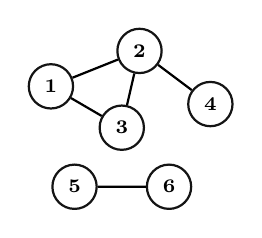
\begin{tikzpicture}[scale=0.75]
        \node[gnode] (1) at (0,1) {1};
        \node[gnode] (2) at (1.5,1.6) {2};
        \node[gnode] (3) at (1.2,0.3) {3};
        \node[gnode] (4) at (2.7,0.7) {4};
        \node[gnode] (5) at (0.4,-0.7) {5};
        \node[gnode] (6) at (2.0,-0.7) {6};
        \draw[thick] (1)--(2) (1)--(3) (2)--(3) (4)--(2) (6)--(5);
      \end{tikzpicture}\\[6pt]
      {\scriptsize\textbf{Directed graph}}\\[2pt]
      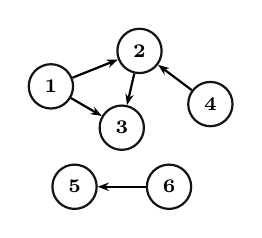
\begin{tikzpicture}[scale=0.75,>={Stealth[length=4pt]}]
        \node[gnode] (1) at (0,1) {1};
        \node[gnode] (2) at (1.5,1.6) {2};
        \node[gnode] (3) at (1.2,0.3) {3};
        \node[gnode] (4) at (2.7,0.7) {4};
        \node[gnode] (5) at (0.4,-0.7) {5};
        \node[gnode] (6) at (2.0,-0.7) {6};
        \draw[thick,->] (1)--(2);
        \draw[thick,->] (1)--(3);
        \draw[thick,->] (2)--(3);
        \draw[thick,->] (4)--(2);
        \draw[thick,->] (6)--(5);
      \end{tikzpicture}
    \end{column}
  \end{columns}
\end{frame}

\begin{frame}{Paths, Cycles, and Degrees}
  \begin{itemize}
    \item \textbf{Path:} A sequence of vertices $(v_1, v_2, \dots, v_k)$ with an edge between each consecutive pair $(v_i, v_{i+1})$. A path is \textbf{simple} if all vertices are distinct.
    \item \textbf{Cycle:} A path of length $\ge 3$ where $v_1 = v_k$ and $v_1, \dots, v_{k-1}$ are distinct.
    \item \textbf{Degree $\deg(v)$:} The number of edges incident to vertex $v$.
      \begin{itemize}
        \item In directed graphs, we split into \textbf{in-degree} $\deg^-(v)$ and \textbf{out-degree} $\deg^+(v)$.
      \end{itemize}
    \item \textbf{Handshaking Lemma:} Every undirected edge contributes $1$ to the degree of both endpoints:
      \[ \sum_{v \in V} \deg(v) = 2|E|. \]
  \end{itemize}
\end{frame}

\begin{frame}{Connectivity, Trees, and Rooted Trees}
  \begin{columns}[c]
    \begin{column}{0.58\textwidth}
      \begin{itemize}
        \item \textbf{Connected Graph:} A path exists between any two vertices $u, v \in V$.
          \begin{itemize}
            \item Maximal connected subgraphs are called \textbf{connected components}.
          \end{itemize}
        \item \textbf{Tree:} A connected, acyclic undirected graph.
          \begin{itemize}
            \item Equivalent: connected with $|E| = |V| - 1$.
            \item Equivalent: \textbf{unique} simple path between any two vertices.
          \end{itemize}
        \item \textbf{Rooted Tree:} Fixing one special \textbf{root} node $r$ orients all edges as $\text{parent} \to \text{child}$.
      \end{itemize}
    \end{column}
    \begin{column}{0.40\textwidth}
      \centering
      {\scriptsize\textbf{Tree rooted at 1}}\\[2pt]
      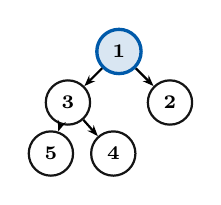
\begin{tikzpicture}[scale=0.72,>={Stealth[length=4pt]}]
        \node[active] (1) at (1.2,1.8) {1};
        \node[gnode] (3) at (0.3,0.9) {3};
        \node[gnode] (2) at (2.1,0.9) {2};
        \node[gnode] (5) at (0.0,0.0) {5};
        \node[gnode] (4) at (1.1,0.0) {4};
        \draw[thick,->] (1)--(3);
        \draw[thick,->] (1)--(2);
        \draw[thick,->] (3)--(5);
        \draw[thick,->] (3)--(4);
      \end{tikzpicture}\\[6pt]
      {\scriptsize\textbf{Same tree rooted at 3}}\\[2pt]
      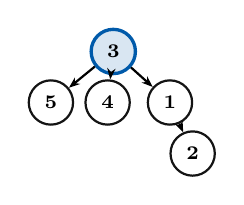
\begin{tikzpicture}[scale=0.72,>={Stealth[length=4pt]}]
        \node[active] (3) at (1.2,1.8) {3};
        \node[gnode] (5) at (0.1,0.9) {5};
        \node[gnode] (4) at (1.1,0.9) {4};
        \node[gnode] (1) at (2.2,0.9) {1};
        \node[gnode] (2) at (2.6,0.0) {2};
        \draw[thick,->] (3)--(5);
        \draw[thick,->] (3)--(4);
        \draw[thick,->] (3)--(1);
        \draw[thick,->] (1)--(2);
      \end{tikzpicture}
    \end{column}
  \end{columns}
\end{frame}

% ============================================================
\section{Storing Graphs: Representations and Trade-Offs}
% ============================================================

\begin{frame}{Three Ways to Represent a Graph}
  \begin{columns}[c]
    \begin{column}{0.26\textwidth}
      \textbf{1. Edge List}\\
      Store $E$ as pairs $(u, v)$:\par\vspace{0.2em}
      {\scriptsize\ttfamily
        2 3\\
        1 2\\
        3 1\\
        3 4\\
        1 5\\
        6 5\par}
    \end{column}
    \begin{column}{0.32\textwidth}
      \centering
      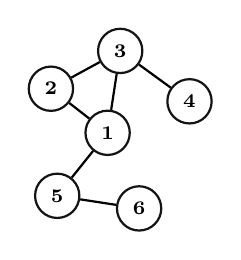
\begin{tikzpicture}[scale=0.8]
        \node[gnode] (3) at (1.3,2.0) {3};
        \node[gnode] (2) at (0.2,1.4) {2};
        \node[gnode] (1) at (1.1,0.7) {1};
        \node[gnode] (4) at (2.4,1.2) {4};
        \node[gnode] (5) at (0.3,-0.3) {5};
        \node[gnode] (6) at (1.6,-0.5) {6};
        \draw[thick] (2)--(3) (1)--(2) (3)--(1) (3)--(4) (1)--(5) (6)--(5);
      \end{tikzpicture}
    \end{column}
    \begin{column}{0.38\textwidth}
      \textbf{2. Adjacency List}\\
      For each $u$, list neighbours:\par\vspace{0.2em}
      {\scriptsize\ttfamily
        1: 2, 3, 5\\
        2: 3, 1\\
        3: 2, 1, 4\\
        4: 3\\
        5: 1, 6\\
        6: 5\par}
    \end{column}
  \end{columns}
  \vspace{0.3em}
  \textbf{3. Adjacency Matrix:} An $N \times N$ table $A$ where $A[u][v] = 1$ if $(u,v) \in E$, else $0$.
\end{frame}

\begin{frame}[fragile]{Adjacency List in Code (C++ and Python)}
  \begin{columns}[t]
    \begin{column}{0.49\textwidth}
      \textbf{C++ (\texttt{vector<int>})}
\begin{lstlisting}[language=C++]
const int MAXN = 100005;
vector<int> g[MAXN];

int main() {
  int n, m;
  cin >> n >> m;
  for (int i = 0; i < m; i++) {
    int u, v;
    cin >> u >> v;
    g[u].push_back(v);
    g[v].push_back(u); // 2-way
  }
}
\end{lstlisting}
    \end{column}
    \begin{column}{0.48\textwidth}
      \textbf{Python (\texttt{list} of \texttt{list}s)}
\begin{lstlisting}[language=Python]
import sys
input = sys.stdin.readline

n, m = map(int, input().split())
g = [[] for _ in range(n + 1)]
for _ in range(m):
  u, v = map(int, input().split())
  g[u].append(v)
  g[v].append(u) # undirected
\end{lstlisting}
      {\scriptsize Total integers stored across all lists: $2|E|$ (or $|E|$ if directed).}
    \end{column}
  \end{columns}
\end{frame}

\begin{frame}[fragile]{Adjacency Matrix in Code}
  \begin{columns}[c]
    \begin{column}{0.52\textwidth}
\begin{lstlisting}[language=C++]
const int MAXN = 1005;
bool g[MAXN][MAXN];

int main() {
    int n, m;
    cin >> n >> m;
    for (int i = 0; i < m; i++) {
        int u, v;
        cin >> u >> v;
        g[u][v] = true;
        g[v][u] = true; // undirected
    }
}
\end{lstlisting}
    \end{column}
    \begin{column}{0.44\textwidth}
      \centering
      {\scriptsize\textbf{Matrix $g[u][v]$ for the 6-node graph}}\\[3pt]
      {\scriptsize
      \begin{tabular}{c|cccccc}
          & 1 & 2 & 3 & 4 & 5 & 6 \\\hline
        1 & 0 & 1 & 1 & 0 & 1 & 0 \\
        2 & 1 & 0 & 1 & 0 & 0 & 0 \\
        3 & 1 & 1 & 0 & 1 & 0 & 0 \\
        4 & 0 & 0 & 1 & 0 & 0 & 0 \\
        5 & 1 & 0 & 0 & 0 & 0 & 1 \\
        6 & 0 & 0 & 0 & 0 & 1 & 0
      \end{tabular}}
      \par\vspace{0.4em}
      {\scriptsize Symmetric ($g[u][v] = g[v][u]$) when undirected.}
    \end{column}
  \end{columns}
\end{frame}

\begin{frame}{Comparison: Memory and Operations}
  \textbf{Memory ($N = |V|$, $E = |E|$):}\par\vspace{0.1em}
  {\scriptsize\setlength{\tabcolsep}{1.8pt}
  \begin{tabular}{lcccc}
    \toprule
    \textbf{Structure} & $N{=}10^3, E{=}10^3$ & $N{=}10^3, E{=}10^5$ & $N{=}5000, E{=}2{\cdot}10^5$ & $N{=}10^5, E{=}2{\cdot}10^5$ \\
    \midrule
    \textbf{Adj.\ List} $O(N{+}E)$ & ${\approx}\,0.01\text{ MB}$ & ${\approx}\,1\text{ MB}$ & ${\approx}\,2\text{ MB}$ & ${\approx}\,2\text{ MB}$ \\
    \textbf{Adj.\ Matrix} $O(N^2)$ & ${\approx}\,1\text{ MB}$ & ${\approx}\,1\text{ MB}$ & ${\approx}\,25\text{ MB}$ & \textcolor{kcpc-red}{\textbf{${\approx}\,10\text{ GB}$}} \\
    \bottomrule
  \end{tabular}}

  \vspace{0.3em}
  \textbf{Operation Time Complexities:}\par\vspace{0.1em}
  {\scriptsize\setlength{\tabcolsep}{3.5pt}
  \begin{tabular}{lccc}
    \toprule
    \textbf{Operation} & \textbf{Adjacency List} & \textbf{Adjacency Matrix} & \textbf{Edge List} \\
    \midrule
    Does edge $(u,v)$ exist? & $O(\deg(u))$ & $O(1)$ & $O(E)$ \\
    Iterate neighbours of $u$ & \textcolor{kcpc-green}{\textbf{$O(\deg(u))$}} & $O(N)$ & $O(E)$ \\
    Inspect all edges & \textcolor{kcpc-green}{\textbf{$O(N + E)$}} & $O(N^2)$ & $O(E)$ \\
    Add / delete edge $(u,v)$ & $O(1)$ / $O(\deg(u))$ & $O(1)$ / $O(1)$ & $O(1)$ / $O(E)$ \\
    Add / delete vertex $u$ & $O(1)$ / $O(N + E)$ & $O(N)$ / $O(N)$ & $O(1)$ / $O(E)$ \\
    \bottomrule
  \end{tabular}}
\end{frame}

\begin{frame}{Try It Yourself: Representations and Degrees}
  Suppose an undirected simple graph has $N = 100\,000$ vertices and $M = 150\,000$ edges.
  \begin{enumerate}
    \item What is the sum of $\deg(v)$ over all $100\,000$ vertices?
    \item If you store the graph in an adjacency list \texttt{g[1..N]}, how many total loop iterations does
      \[ \texttt{for } u = 1 \dots N: \quad \texttt{for } v \text{ in } g[u]: \dots \]
      perform, and why is this much faster than scanning an adjacency matrix?
    \item Can an undirected simple graph on $5$ vertices have vertex degrees $3, 3, 3, 2, 2$?
  \end{enumerate}
  \emph{Discuss with a neighbour; full solutions are at the end of the slides.}
\end{frame}

% ============================================================
\section{Breadth-First Search (BFS) and Unweighted Shortest Paths}
% ============================================================

\begin{frame}{Breadth-First Search (BFS): Layer-by-Layer Exploration}
  \begin{columns}[c]
    \begin{column}{0.51\textwidth}
      \textbf{Core Idea:}
      \begin{itemize}
        \item Start at source vertex $s$ (layer $0$).
        \item Visit all neighbours at distance $1$, then distance $2$, then distance $3$, and so on.
        \item Maintain a \textbf{FIFO queue} $q$ of discovered vertices whose neighbours still need to be inspected.
        \item Mark a vertex \texttt{visited} \textbf{as soon as it is pushed} into $q$ so it is never enqueued twice.
      \end{itemize}
    \end{column}
    \begin{column}{0.46\textwidth}
      \centering
      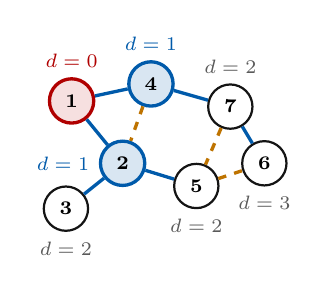
\begin{tikzpicture}[scale=0.72]
        \node[done,label={[font=\scriptsize,text=kcpc-red]above:$d=0$}] (1) at (0,1.6) {1};
        \node[active,label={[font=\scriptsize,text=kcpc-blue]above:$d=1$}] (4) at (1.4,1.9) {4};
        \node[active,label={[font=\scriptsize,text=kcpc-blue]left:$d=1$}] (2) at (0.9,0.5) {2};
        \node[gnode,label={[font=\scriptsize,text=kcpc-muted]below:$d=2$}] (3) at (-0.1,-0.3) {3};
        \node[gnode,label={[font=\scriptsize,text=kcpc-muted]above:$d=2$}] (7) at (2.8,1.5) {7};
        \node[gnode,label={[font=\scriptsize,text=kcpc-muted]below:$d=2$}] (5) at (2.2,0.1) {5};
        \node[gnode,label={[font=\scriptsize,text=kcpc-muted]below:$d=3$}] (6) at (3.4,0.5) {6};
        \draw[treeedge] (1)--(4) (1)--(2) (4)--(7) (2)--(3) (2)--(5) (7)--(6);
        \draw[backedge] (4)--(2) (7)--(5) (5)--(6);
      \end{tikzpicture}
      \\[3pt]
      {\scriptsize Solid blue: \textbf{BFS tree edges}; dashed: \textbf{cross edges}.}
    \end{column}
  \end{columns}
\end{frame}

\begin{frame}{BFS Step-by-Step Walkthrough}
  Using the adjacency list from the previous slide starting at vertex $1$:\par\vspace{0.2em}
  {\scriptsize\setlength{\tabcolsep}{3.2pt}
  \begin{tabular}{clll}
    \toprule
    \textbf{Pop $v$} & \textbf{List $g[v]$} & \textbf{Newly Discovered ($d[u] = d[v]+1$)} & \textbf{Queue $q$} \\
    \midrule
    Init & --- & Push $1$ ($d[1]=0$) & $[1]$ \\
    $1$ & $4, 2$ & Push $4, 2$ ($d=1, \text{par}=1$) & $[4, 2]$ \\
    $4$ & $1, 2, 7$ & $1,2$ already visited; push $7$ ($d=2, \text{par}=4$) & $[2, 7]$ \\
    $2$ & $1, 3, 5, 4$ & Push $3, 5$ ($d=2, \text{par}=2$) & $[7, 3, 5]$ \\
    $7$ & $4, 5, 6$ & Push $6$ ($d=3, \text{par}=7$) & $[3, 5, 6]$ \\
    $3, 5, 6$ & all visited & None & $[]$ (done) \\
    \bottomrule
  \end{tabular}}
  \vspace{0.3em}
  \begin{itemize}
    \item Discovery order: $\mathbf{1, 4, 2, 7, 3, 5, 6}$, with distances $d = [0, 1, 1, 2, 2, 2, 3]$.
  \end{itemize}
\end{frame}

\begin{frame}[fragile]{BFS with Shortest Paths and Parent Reconstruction}
  \begin{columns}[t]
    \begin{column}{0.48\textwidth}
      \textbf{C++ Implementation}
\begin{lstlisting}[language=C++]
vector<int> dist(n + 1, -1);
vector<int> parent(n + 1, 0);
queue<int> q;
q.push(start);
dist[start] = 0;

while (!q.empty()) {
  int v = q.front();
  q.pop();
  for (int u : g[v]) {
    if (dist[u] == -1) {
      dist[u] = dist[v] + 1;
      parent[u] = v;
      q.push(u);
    }
  }
}
\end{lstlisting}
    \end{column}
    \begin{column}{0.49\textwidth}
      \textbf{Properties of BFS:}
      \begin{itemize}
        \item Tree edges form a \textbf{shortest-path tree} rooted at \texttt{start}.
        \item Every vertex is enqueued at most once and each edge is inspected twice: $\mathbf{O(N + E)}$ time and space.
        \item \textbf{Path reconstruction} (\emph{Message Route}): follow \texttt{cur = parent[cur]} from target $t$ back to \texttt{start}, then reverse.
      \end{itemize}
    \end{column}
  \end{columns}
\end{frame}

\begin{frame}{Try It Yourself: BFS Shortest Path}
  Consider the 7-vertex graph from the BFS walkthrough (edges: $(1,4), (1,2), (4,2), (4,7), (2,3), (2,5), (7,5), (7,6), (5,6)$).
  \begin{enumerate}
    \item What is the shortest distance \texttt{dist[6]} from vertex $1$ to vertex $6$, and what is the parent chain \texttt{6 -> parent[6] -> ... -> 1}?
    \item Why is the edge $(5, 6)$ a \textbf{cross edge} rather than a tree edge when $7$ is popped before $5$?
    \item What bug occurs if you set \texttt{visited[u] = true} when \emph{popping} $u$ from the queue instead of when \emph{pushing} $u$?
  \end{enumerate}
\end{frame}

% ============================================================
\section{Depth-First Search (DFS) and Edge Classification}
% ============================================================

\begin{frame}[fragile]{Depth-First Search (DFS): Plunge and Backtrack}
  \begin{columns}[c]
    \begin{column}{0.52\textwidth}
      \textbf{Core Idea:}
      \begin{itemize}
        \item Follow one branch as deep as possible until stuck, then \textbf{backtrack}.
        \item Naturally expressed via recursion (or an explicit LIFO stack).
      \end{itemize}
\begin{lstlisting}[language=C++]
void dfs(int v) {
    vis[v] = true;
    tin[v] = ++timer;
    for (int u : g[v]) {
        if (!vis[u]) {
            dfs(u);
        }
    }
    tout[v] = ++timer;
}
\end{lstlisting}
    \end{column}
    \begin{column}{0.45\textwidth}
      \centering
      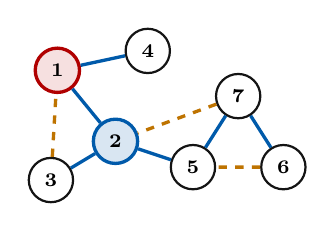
\begin{tikzpicture}[scale=0.82]
        \node[done] (1) at (0,1.6) {1};
        \node[gnode] (4) at (1.4,1.9) {4};
        \node[active] (2) at (0.9,0.5) {2};
        \node[gnode] (3) at (-0.1,-0.1) {3};
        \node[gnode] (7) at (2.8,1.2) {7};
        \node[gnode] (5) at (2.1,0.1) {5};
        \node[gnode] (6) at (3.5,0.1) {6};
        \draw[treeedge] (1)--(4) (1)--(2) (2)--(3) (2)--(5) (5)--(7) (7)--(6);
        \draw[backedge] (3)--(1) (7)--(2) (6)--(5);
      \end{tikzpicture}
      \\[4pt]
      {\scriptsize
      \textbf{DFS Entry (\texttt{tin}) order:} $1, 4, 2, 3, 5, 7, 6$\\
      \textbf{DFS Exit (\texttt{tout}) order:} $4, 3, 6, 7, 5, 2, 1$}
    \end{column}
  \end{columns}
\end{frame}

\begin{frame}{DFS Properties and Edge Classification}
  \begin{itemize}
    \item \textbf{Subtree Property:} Once DFS exits vertex $v$, it has visited \emph{every} vertex reachable from $v$ along unvisited paths. Vertex $u$ is in $v$'s DFS subtree iff $\text{tin}[v] \le \text{tin}[u] \le \text{tout}[u] \le \text{tout}[v]$.
    \item \textbf{Edge Types in Undirected Graphs:} Every edge is either:
      \begin{enumerate}
        \item a \textbf{Tree Edge} (discovers a new vertex $u$ from $v$), or
        \item a \textbf{Back Edge} (connects $v$ to an already-visited ancestor $u \neq \text{parent}[v]$).
      \end{enumerate}
    \item \textbf{Edge Types in Directed Graphs:} In addition to tree and back edges, directed graphs can have \textbf{forward edges} (to a proper descendant) and \textbf{cross edges} (to a previously finished branch).
    \item \textbf{Complexity:} Visits every vertex and edge once: $\mathbf{O(N + E)}$ time and $\mathbf{O(N)}$ recursion stack.
  \end{itemize}
\end{frame}

\begin{frame}{Try It Yourself: DFS Trace and Back-Edges}
  In the 7-vertex DFS walkthrough graph, the adjacency lists are:
  \begin{center}
    {\small $1:[4,2,3],\quad 2:[1,3,5,7],\quad 3:[2,1],\quad 4:[1],$\\[2pt]
    $5:[2,7,6],\quad 6:[7,5],\quad 7:[2,5,6].$}
  \end{center}
  \begin{enumerate}
    \item When DFS is at vertex $3$ (called from $2$, which was called from $1$), it inspects neighbour $1$. Why does $(3, 1)$ prove the existence of a simple cycle?
    \item List all three back-edges encountered during $\texttt{dfs}(1)$ and the simple cycle each back-edge closes.
  \end{enumerate}
\end{frame}

% ============================================================
\section{Core Algorithmic Patterns for the Problem Sheet}
% ============================================================

\begin{frame}{Pattern 1: Finding Connected Components}
  \begin{itemize}
    \item Loop through vertices $i = 1, \dots, n$.
    \item Whenever $i$ is unvisited, start DFS or BFS from $i$. This traversal visits exactly the vertices in $i$'s connected component.
    \item Record $i$ as that component's representative and continue scanning.
  \end{itemize}

  \vspace{0.6em}
  \textbf{Application --- Building Roads:}
  If the graph has $C$ components represented by $r_1, \dots, r_C$, add roads
  \[(r_1,r_2), (r_2,r_3), \dots, (r_{C-1},r_C).\]
  Each road joins two components, so $C-1$ roads are sufficient and necessary.

  \vspace{0.4em}
  \textbf{Complexity:} $O(N+E)$ time with an adjacency list.
\end{frame}

\begin{frame}{Pattern 2: Recognising Cyclic Components}
  \begin{columns}[c]
    \begin{column}{0.56\textwidth}
      \textbf{Theorem:} A connected component of a simple undirected graph is a simple cycle if and only if every vertex in it has degree $2$.
      \begin{itemize}
        \item A cycle gives every vertex exactly two incident edges.
        \item Conversely, in a finite connected component where every vertex has degree $2$, following edges must eventually return to the start. Connectivity rules out vertices outside that cycle.
      \end{itemize}
    \end{column}
    \begin{column}{0.40\textwidth}
      \centering
      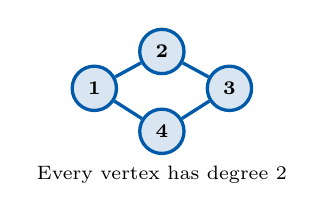
\begin{tikzpicture}[scale=0.78]
        \node[active] (a) at (0,0.9) {1};
        \node[active] (b) at (1.1,1.5) {2};
        \node[active] (c) at (2.2,0.9) {3};
        \node[active] (d) at (1.1,0.2) {4};
        \draw[treeedge] (a)--(b)--(c)--(d)--(a);
        \node[font=\scriptsize] at (1.1,-0.5) {Every vertex has degree 2};
      \end{tikzpicture}
    \end{column}
  \end{columns}
\end{frame}

\begin{frame}{Pattern 2: Applying the Degree Test}
  \textbf{Goal:} Count connected components that are simple cycles.
  \begin{enumerate}
    \item For each unvisited vertex, traverse its entire component.
    \item Check whether every vertex in the component has degree $2$.
    \item Count the component if and only if that check succeeds.
  \end{enumerate}
  The traversal ensures the component is connected; the degree test then characterises a cycle.\\[0.4em]
  \textbf{Complexity:} $O(N+E)$ for the whole graph.
\end{frame}

\begin{frame}{Pattern 3: Finding Cycles in Undirected Graphs}
  \textbf{Application --- Round Trip:} During DFS, track each vertex's parent.
  \begin{enumerate}
    \item If an edge from $v$ discovers an unvisited neighbour $u$, set $\texttt{parent}[u]=v$ and continue DFS.
    \item Ignore the edge back to $\texttt{parent}[v]$; it is just the same undirected edge in reverse.
    \item If $u$ is already visited and $u \neq \texttt{parent}[v]$, the edge $(v,u)$ closes a cycle with the tree path from $u$ to $v$.
  \end{enumerate}
  Reconstruct the cycle by following parent pointers from $v$ back to $u$.
  \[\text{Traversal and reconstruction take }O(N+E)\text{ time.}\]
\end{frame}

\begin{frame}{Pattern 4: Functional Graphs}
  \textbf{Definition:} A functional graph is a directed graph where every vertex has exactly one outgoing edge, $u \to f(u)$.
  \begin{itemize}
    \item Following edges from any starting vertex eventually reaches a directed cycle.
    \item Each component consists of one directed cycle with trees feeding into its cycle vertices (a $\rho$-shape).
    \item \textbf{Badge:} Repeatedly follow the successor until a vertex is visited twice; that repeated vertex is the first student receiving a second hole.
    \item \textbf{Game on Axis:} Treat out-of-bounds jumps as edges to a terminal sink $0$. In the reversed graph, the vertices that terminate form a tree rooted at $0$.
  \end{itemize}
\end{frame}

\begin{frame}{Pattern 5: Bipartite Graphs}
  \begin{columns}[c]
    \begin{column}{0.56\textwidth}
      \textbf{Definition (\emph{Building Teams}):}
      A graph is \textbf{bipartite} if its vertices can be split into two teams so every edge connects opposite teams.

      \vspace{0.4em}
      \textbf{Theorem:} A graph is bipartite if and only if it has no odd-length cycle.
      \begin{itemize}
        \item Even cycles alternate colours consistently.
        \item An odd cycle eventually requires one edge to connect vertices of the same colour.
      \end{itemize}
    \end{column}
    \begin{column}{0.40\textwidth}
      \centering
      {\scriptsize\textbf{Bipartite: even cycle $C_4$}}\\[2pt]
      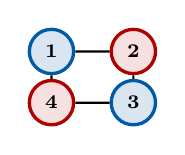
\begin{tikzpicture}[scale=0.65]
        \node[active] (1) at (0,1) {1};
        \node[done] (2) at (1.6,1) {2};
        \node[active] (3) at (1.6,0) {3};
        \node[done] (4) at (0,0) {4};
        \draw[thick] (1)--(2)--(3)--(4)--(1);
      \end{tikzpicture}\\[5pt]
      {\scriptsize\textbf{Not bipartite: odd cycle $C_3$}}\\[2pt]
      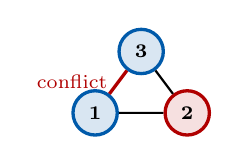
\begin{tikzpicture}[scale=0.65]
        \node[active] (1) at (0,0) {1};
        \node[done] (2) at (1.8,0) {2};
        \node[active] (3) at (0.9,1.2) {3};
        \draw[thick] (1)--(2)--(3);
        \draw[very thick,kcpc-red] (3)--(1) node[midway,left,font=\scriptsize] {conflict};
      \end{tikzpicture}
    \end{column}
  \end{columns}
\end{frame}

\begin{frame}{Pattern 6: 2-Colouring with BFS or DFS}
  \begin{enumerate}
    \item For each uncoloured vertex $s$, set $\texttt{col}[s]=1$ and start BFS/DFS.
    \item For each edge $(v,u)$:
      \begin{itemize}
        \item If $\texttt{col}[u]=0$, assign the opposite colour: $\texttt{col}[u]=3-\texttt{col}[v]$.
        \item If $\texttt{col}[u]=\texttt{col}[v]$, the graph is not bipartite; output \texttt{IMPOSSIBLE}.
      \end{itemize}
    \item Repeat from every uncoloured vertex so disconnected components are also checked.
  \end{enumerate}
  \textbf{Complexity:} $O(N+E)$ time and $O(N+E)$ space with an adjacency list.
\end{frame}

\begin{frame}{Pattern 7: Tree Diameter in Two Traversals}
  \textbf{Problem (\emph{Tree Diameter}):} Find the maximum distance between any two nodes in a tree, without dynamic programming.
  \begin{enumerate}
    \item Pick an arbitrary vertex $r$ and run BFS/DFS to find a farthest vertex $u$.
    \item Run a second BFS/DFS from $u$ to find a farthest vertex $v$.
    \item The distance $\text{dist}(u,v)$ is the tree diameter.
  \end{enumerate}
  \textbf{Why it works:} Paths in a tree are unique. The farthest vertex from an arbitrary root is an endpoint of a longest path; the second traversal reaches the other endpoint.

  \vspace{0.3em}
  \textbf{Complexity:} Two linear traversals take $O(N)$ time and $O(N)$ space.
\end{frame}

\begin{frame}{Pattern 8: Topological Sorting a DAG}
  A \textbf{Directed Acyclic Graph (DAG)} has no directed cycles. Its vertices can be ordered so every edge $u \to v$ goes forward in the order.

  \vspace{0.4em}
  \textbf{Kahn's Algorithm (BFS):}
  \begin{enumerate}
    \item Compute the in-degree $\texttt{indeg}[v]$ of every vertex.
    \item Add every vertex with in-degree $0$ to a queue.
    \item Pop $u$, append it to the order, and decrement the in-degree of each outgoing neighbour $v$.
    \item Whenever $\texttt{indeg}[v]$ reaches $0$, add $v$ to the queue.
  \end{enumerate}
  Each vertex and edge is processed once, so the algorithm takes $O(N+E)$ time. If fewer than $N$ vertices are output, the graph contains a directed cycle.
\end{frame}

\begin{frame}{Pattern 9: Dynamic Programming on a DAG}
  A topological order ensures that when a vertex is processed, all contributions from its predecessors have already been calculated.

  \vspace{0.5em}
  \textbf{Counting paths (\emph{DAG Number of Routes}):}
  Set $\text{dp}[1]=1$. For each edge $u \to v$ in topological order, add $\text{dp}[u]$ to $\text{dp}[v]$ modulo $10^9+7$.

  \[\text{dp}[v] = \sum_{u \to v} \text{dp}[u] \pmod{10^9+7}.\]

  \textbf{Longest path (\emph{AtCoder DP G}):} Process vertices in reverse topological order and use
  \[\text{dp}[u] = \max_{u \to v}(1 + \text{dp}[v]),\]
  with $\text{dp}[u]=0$ for a sink. Both algorithms run in $O(N+E)$ time.
\end{frame}

\begin{frame}{Pattern 10: Auxiliary Graph Modelling (\emph{Rudolf and Subway})}
  \begin{columns}[c]
    \begin{column}{0.56\textwidth}
      \textbf{Challenge:} Riding tracks of the same colour costs one ticket. Joining every pair of stations on one colour directly can create $O(N^2)$ edges.

      \vspace{0.3em}
      \textbf{Star expansion:}
      \begin{itemize}
        \item Create an auxiliary vertex $L_c$ for each colour $c$.
        \item Replace every track $(u,v,c)$ by edges $u-L_c$ and $v-L_c$.
        \item Riding one line from station $u$ to station $v$ corresponds to $u \to L_c \to v$.
      \end{itemize}
    \end{column}
    \begin{column}{0.41\textwidth}
      \centering
      {\scriptsize\textbf{Station and colour vertices}}\\[4pt]
      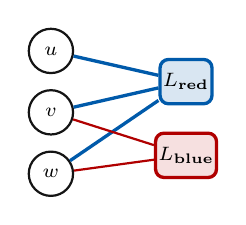
\begin{tikzpicture}[scale=0.78]
        \node[gnode] (s1) at (0,1.6) {$u$};
        \node[gnode] (s2) at (0,0.6) {$v$};
        \node[gnode] (s3) at (0,-0.4) {$w$};
        \node[active,rectangle,rounded corners=3pt] (c1) at (2.2,1.1) {$L_{\text{red}}$};
        \node[done,rectangle,rounded corners=3pt] (c2) at (2.2,-0.1) {$L_{\text{blue}}$};
        \draw[treeedge] (s1)--(c1) (s2)--(c1) (s3)--(c1);
        \draw[thick,kcpc-red] (s2)--(c2) (s3)--(c2);
      \end{tikzpicture}
    \end{column}
  \end{columns}

  \vspace{0.2em}
  Run BFS from $b$ to $e$ in the expanded graph; the answer is $\text{dist}(b,e)/2$. The expanded graph has $O(N+M)$ vertices and edges.
\end{frame}

\begin{frame}{Try It Yourself: Tree Bipartiteness}
  Can a tree with $N \ge 2$ vertices fail to be bipartite? Explain why or why not.

  \vspace{0.8em}
  \emph{Hint: Consider the parity of each vertex's depth from a chosen root.}
\end{frame}

\begin{frame}{Try It Yourself: Counting Paths in a DAG}
  Suppose a DAG has vertices $\{1,2,3,4\}$ and directed edges
  \[1 \to 2,\quad 1 \to 3,\quad 2 \to 3,\quad 2 \to 4,\quad 3 \to 4.\]
  Find a valid topological ordering and calculate the number of directed paths from vertex $1$ to vertex $4$.
\end{frame}

\begin{frame}{Try It Yourself: Longest Path in a DAG}
  Using the same DAG, find the length (number of edges) of the longest directed path from vertex $1$ to vertex $4$.

  \vspace{0.8em}
  \emph{Hint: Compare the direct routes with the route that passes through both vertices $2$ and $3$.}
\end{frame}

% ============================================================
\section{Conclusion}
% ============================================================

\begin{frame}{Summary: Matching Problems to Graph Techniques}
  \centering
  {\scriptsize\setlength{\tabcolsep}{3pt}
  \begin{tabular}{lll}
    \toprule
    \textbf{Problem Goal} & \textbf{Key Structure / Invariant} & \textbf{Algorithm} \\
    \midrule
    Connect components & Reachability equivalence classes & DFS/BFS, $O(N{+}E)$ \\
    Shortest unweighted route & Layer-by-layer distance & BFS + \texttt{parent[]}, $O(N{+}E)$ \\
    Find undirected cycle & Back-edge to $u \neq \texttt{parent}[v]$ & DFS + \texttt{parent[]}, $O(N{+}E)$ \\
    Split into two teams & Bipartite $\iff$ no odd cycle & 2-colouring, $O(N{+}E)$ \\
    Component is a cycle & Connected and $\forall v, \deg(v) = 2$ & Degree check, $O(N{+}E)$ \\
    Paths / longest in DAG & Acyclic $\implies$ topological order & Kahn / DFS DP, $O(N{+}E)$ \\
    Tree diameter (no DP) & Farthest node is diameter end & Two-BFS/DFS, $O(N)$ \\
    Same-colour line rides & Star expansion with nodes $L_c$ & Auxiliary BFS, $O(N{+}E)$ \\
    \bottomrule
  \end{tabular}}
\end{frame}

% ============================================================
% Appendix: Worked Answers to Interactive Checkpoints
% ============================================================

\begin{frame}{Try It Yourself: Representations and Degrees (Answers)}
  \begin{enumerate}
    \item \textbf{Sum of degrees:} By the Handshaking Lemma,
      \[ \sum_{v=1}^{100\,000} \deg(v) = 2M = 2 \times 150\,000 = 300\,000. \]
    \item \textbf{Adjacency list loop iterations:} The inner loop runs $\deg(u)$ times for vertex $u$, so total iterations equal $\sum_u \deg(u) = 300\,000$ ($3 \times 10^5$ operations), compared to $N^2 = 10^{10}$ operations in an adjacency matrix.
    \item \textbf{Degree sequence $3, 3, 3, 2, 2$:} Impossible! Their sum is $3+3+3+2+2 = 13$, which is odd, violating $\sum \deg(v) = 2|E|$.
  \end{enumerate}
\end{frame}

\begin{frame}{Try It Yourself: BFS Shortest Path (Answers)}
  \begin{enumerate}
    \item \textbf{Shortest path to $6$:} $\texttt{dist}[6] = 3$. Following parents gives $6 \leftarrow 7 \leftarrow 4 \leftarrow 1$, so the shortest path is $1 \to 4 \to 7 \to 6$.
    \item \textbf{Why $(5, 6)$ is a cross edge:} Both $7$ and $5$ are in layer $d = 2$, with $7$ enqueued before $5$. When $7$ is popped, it discovers $6$ ($d[6] = 3$). Later, when $5$ is popped, $6$ is already visited, so $(5, 6)$ is a non-tree cross edge.
    \item \textbf{Marking visited on pop instead of push:} The same vertex can be pushed into the queue multiple times by different neighbours in the previous layer, causing duplicate work and up to $O(E)$ queue blowup (and incorrect parent overwrites).
  \end{enumerate}
\end{frame}

\begin{frame}{Try It Yourself: DFS Trace and Back-Edges (Answers)}
  \begin{enumerate}
    \item \textbf{Why $(3, 1)$ proves a cycle:} At vertex $3$, $\texttt{parent}[3] = 2$. Neighbour $1$ is already visited and $1 \neq \texttt{parent}[3]$, so $1$ is an ancestor of $3$ in the DFS tree. Combining the tree path $1 \to 2 \to 3$ with the back-edge $(3, 1)$ gives the simple cycle $1 - 2 - 3 - 1$.
    \item \textbf{All three back-edges:}
      \begin{itemize}
        \item $(3, 1)$ closes cycle $1 - 2 - 3 - 1$.
        \item $(7, 2)$ closes cycle $2 - 5 - 7 - 2$.
        \item $(6, 5)$ closes cycle $5 - 7 - 6 - 5$.
      \end{itemize}
  \end{enumerate}
\end{frame}

\begin{frame}{Try It Yourself: Tree Bipartiteness (Answer)}
  \textbf{Yes.} Root the tree anywhere and colour each vertex by the parity of its depth.

  Every tree edge joins a parent to a child, whose depths differ by exactly one, so its endpoints have opposite colours. Thus this is a valid 2-colouring. Equivalently, a tree has no cycles, and hence no odd cycles.
\end{frame}

\begin{frame}{Try It Yourself: Counting DAG Paths (Answer)}
  A valid topological ordering is $[1,2,3,4]$. Initialise $\text{dp}[1]=1$ and process the edges in that order:
  \begin{align*}
    \text{dp}[2] &= 1,\\
    \text{dp}[3] &= \text{dp}[1]+\text{dp}[2]=2,\\
    \text{dp}[4] &= \text{dp}[2]+\text{dp}[3]=1+2=\mathbf{3}.
  \end{align*}
  The three routes are $1\to2\to4$, $1\to3\to4$, and $1\to2\to3\to4$.
\end{frame}

\begin{frame}{Try It Yourself: Longest DAG Path (Answer)}
  The longest route is $1\to2\to3\to4$, which contains \textbf{3 edges}.

  The other routes are $1\to2\to4$ and $1\to3\to4$, each with 2 edges. Therefore the longest-path answer is $3$.
\end{frame}

\end{document}
